%----------------------------------------------------------------------
%                        PROJECT DEFINITION
%----------------------------------------------------------------------
\renewcommand{\projnr}{B2}
\renewcommand{\projtitleshort}{Influence of multiple collisions}
\renewcommand{\projauth}{Wurm, Blum}
%
\setcounter{section}{0}
\noindent{\normalfont\sffamily\Large\bfseries Project \projnr: \projtitleshort}
%
\section{Full title:}
\hspace{1\baselineskip}\\
\centerline{\large ``The influence of multiple collisions on the evolution of dusty bodies''}
%\centerline{\large and the efficiency of electrostatic secondary agglomeration''}
%
\section{General information}\mbox{}
\subsection{Principle investigators:}
\hspace{-\baselineskip}\\\noindent
%
{\bfseries\itshape Wurm}, Gerhard, Dr.\\
Emmy Noether Reserach group, non-tenure\\
Date-of-birth: 05. April 1967, Nationality: German\\
DFG Code number of latest application: WU 321/2-4\\
Institut f\"ur Planetologie\\
Wilhelm-Klemm-Str.~10\\
48149 M\"unster\\
Tel: 0251 8339052\\
Fax: 0251 8336301\\
E-mail: gwurm@uni-muenster.de\\
Private address: Kesslerweg 50d, 48155 M\"unster, Tel: 0251 6279418\\
%
\vspace{1em}\\\noindent
{\bfseries\itshape Blum}, J\"urgen, Prof.~Dr.\\
C3, tenure\\
Date-of-birth: 05. April 1962, Nationality: German\\
DFG Code number of latest application: Bl 298-6/2\\
Institut f\"ur Geophysik und extraterrestrische Physik\\
Mendelssohnstr.~3\\
38106 Braunschweig\\
Tel: 0531 391 5217\\
Fax: 0531 391 8126\\
Email: j.blum@tu-bs.de\\
Private address: Wendenring 14, 38114 Braunschweig, Tel: 0531 1216432\\

\subsection{Co-investigators within this Forschergruppe:}
\begin{coilist}
\item O.~Krau{\ss} (IFP, Univ. M\"unster)
\item W.~Kley (TAT/CPT, Univ. T\"ubingen)
\item H.~Klahr (MPIA, Heidelberg)
\end{coilist}


\newpage

\section{Summary (Zusammenfassung)}
\subsubsection{Summary:}
The experimental data on the outcome of individual collisions with respect to planetesimal formation
is steadily growing. However, all the
work done so far assumes a certain simple initial state of two colliding bodies based on
more or less plausible assumptions. It is unknown how a target evolves over a
large number of collisions. Therefore, this project aims at understanding the self-consistent evolution
of an individual large dusty body under the influence of multiple impacts. The
role of compaction, loosening, fragmentation, elastic waves, ejection and
re-accretion of material will be studied. The project uses impact
experiments, models for individual collisions, and numerical calculations of
gas flow through porous bodies for re-accretion of fragments.

\subsubsection{Zusammenfassung:}
Die experimentelle Untersuchungen von St\"o{\ss}en einzelner K\"orper liefert stetig neue Daten \"uber den Ausgang 
von Kollisionen im Hinblick auf Planetesimalbildung. Bislang werden die Anfangsbedingungen
f\"ur die Struktur der sto{\ss}enden K\"orper allerdings
vor\-ge\-geben. Es ist derzeit nicht klar, wie sich ein K\"orper \"uber eine Vielzahl von St\"o{\ss}en hinweg
selbstkonsistent entwickelt. Ziel des Projekts ist es daher, die selbstkonsistente Entwicklung eines
K\"orpers unter
dem Einflu{\ss} sukzessiver Impakte zu verstehen. Hierbei werden die Bedeutung von Kompaktierung,
Auflockerung, Fragmentation, elastischen Wellen wie auch der Auswurf von Ejekta und die
Reakkretierung von Material untersucht. Es werden sowohl Experimente als auch
numerische Rechnungen verwendet. Letztere beinhalten die Simulation von St\"o{\ss}en und die numerische
Behandlung m\"oglicher
Reakkretion von Fragmenten durch Gasfluss durch einen por\"osen K\"orper.

\section{State of the art (Stand der Forschung)}

It is widely assumed that km-size planetesimals form by successive
collisions of smaller bodies in protoplanetary disks (Weidenschilling \&
Cuzzi~1993).  During planetesimal formation it is inevitable that
high-velocity collisions ($>50$ m/s) take place, in which small bodies ($<
10$ cm) collide with larger ones ($> 10$ cm) (Weidenschilling \&
Cuzzi~1993; Sekiya \& Takeda~2003). Early experimental work on impacts
into regolith was done by Hartmann ~(1978).  In ground based experiments a
solid impactor buried itself into the target regolith. This was initially
taken as evidence that large dusty bodies will stick in high speed
collisions at several tens of m/s. Colwell \& Taylor ~(1999) and Colwell
~(2003) revealed in microgravity experiments that an impactor rather bounces
off and that burial of the projectile was due to gravity, which masked the
rebound in the earlier ground based experiments by Hartmann ~(1978).  The
experiments by Colwell (2003) showed that only slow collisions below 20 cm/s
resulted in sticking of the solid projectile. Collisions with ice particles
by Bridges et al.~(1996) also suggested that no sticking of icy particles
would occur above a few cm/s collision velocity. Further evidence that
collisions at velocities above a few m/s are non-constructive came from
experiments on organic matter by Kouchi et al.~(2002). Even though the
material was rather sticky, no sticking of mm-size particles could be
observed above 5m/s collision velocity.  Only recently experiments showed
that high-velocity collisions can lead to mass gain if both colliding
particles are compact dust aggregates (Wurm et al.~2005b). In fact high
collision velocities might prove better for growth than medium velocity
collisions. Thus there might be different velocity regimes in which
collisions can lead to sticking or fragmentation and the details depend on
other parameters of the colliding bodies like size, porosity, material. In
summary the question which is the outcome of an individual collision depends
strongly on the morphology of the colliding bodies.  Therefore, the
morphological evolution of a larger body has strong relevance to the
question if -- and how -- planetesimals form by aggregation of smaller
bodies. This is sketched in figure \ref{Schema}.

\begin{figure}
%\centerline{\includegraphics[width=15cm]{sketch.eps}}
\centerline{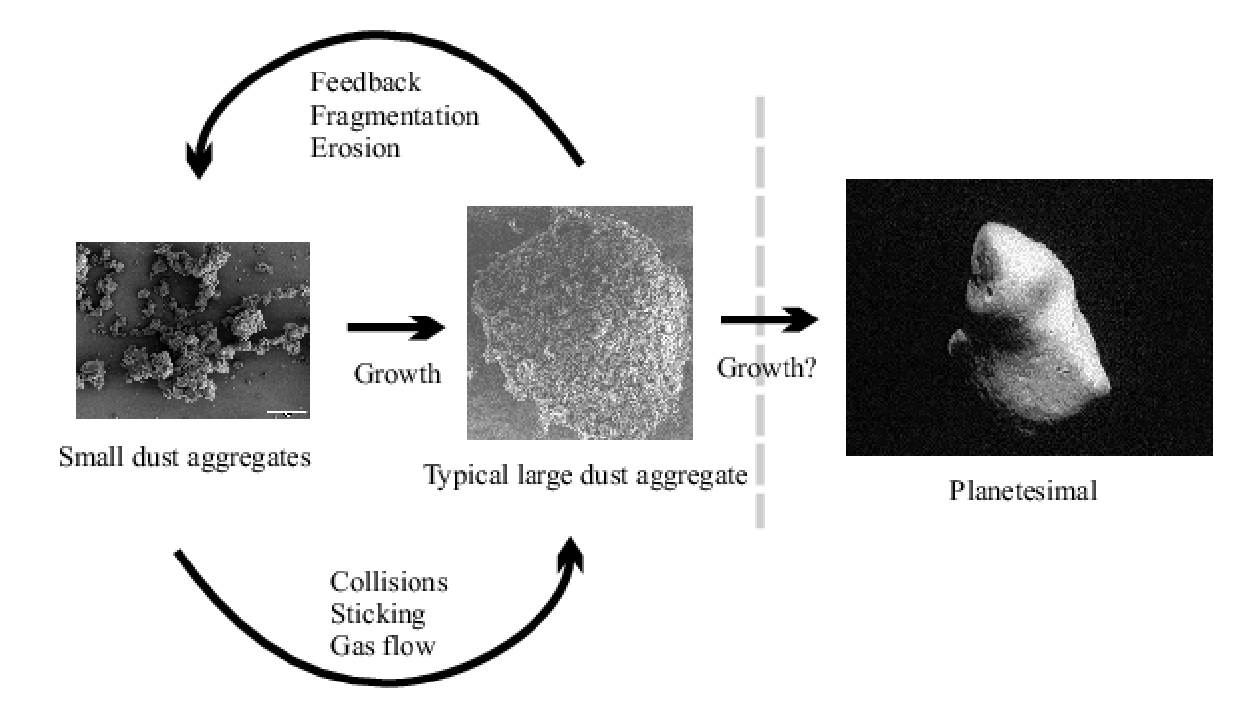
\includegraphics[width=15cm]{b2fig1.eps}}
\caption{\label{Schema}The central role of large dust aggregates of 
dm to m-size. If collisions with smaller particles on average can lead to
further growth, planetesimals might form. If collisions are disruptive in
most cases, planetesimal growth would be inhibited. In that case the typical
large aggregate would still dominate the (observable) dust distribution by
feeding smaller dust aggregates back to the disk.}
\end{figure}


Here, in a first step 'large' refers to dm to m-size bodies, since these
will collide most frequently with smaller dust aggregates due to the high
relative velocities and presumably play a dominant role in the circle of
dust recycling by growth and fragmentation. While for well-defined
parameters individual impacts have been and are simulated in the laboratory,
no self-consistent prediction of the evolution of dusty bodies has been made
yet. Numerical calculations on the evolution of the size distribution of an
evolving system of colliding particles have been carried out
(Weidenschilling 1997; Dullemond \& Dominik 2005).  These calculations
are -- so far -- based on ad hoc assumptions of sticking or fragmentation.
However, as multiple impacts occur they will gradually alter the shape and
structure (e.g.~compactness, surface, inner pore sizes) of a target body and
the outcome of the n-th collision of an evolving body is unknown and ad hoc
assumptions are currently the only way to proceed with calculations. It is
thus of fundamental importance to get a better restriction on how a growing
body evolves in morphology.

Static compression of dust aggregates leads to their compaction (Blum \&
Schr\"apler 2004b).  This does not necessarily mean that a collision will
also lead to a compaction of the colliding dust aggregates. It is found in
granular media research that local pressure can lead to a density decrease
on a larger scale. This is known as Reynolds principle of dilatancy
(Reynolds 1885).  It is also possible that a dusty body is only compacted
locally by an impact but gets decompacted on a larger scale. This has
recently been observed in drop tower experiments (Krauss et al.\ unpublished
data). In collisions onto porous target bodies, elastic waves can also eject
particles (Wurm et al.~2005a) which might be re-accreted by gas flow (Wurm et
al.~2001, 2004; Sekiya \& Takeda 2003). Such a gas flow (head wind) of up to
about 50m/s is always present for large objects due to the different motion
between the gas (sub-Keplerian) and the solids, for both cases of laminar
and turbulent disk flow (Weidenschilling 1993; Sekiya \& Takeda 2003;
Klahr et al.~2006).  The interaction of particle ejecta and gas flow is
further linked to the question on gas flow {\it through} the body which for
large porosities can be significant. It can help re-accrete small ejected
particles more efficiently if not at all (Wurm et al.~2004).  Growth and
erosion of a primary impact depend on the morphology of the colliding
bodies.  The gas flow through a body also depends on the morphology, so
morphology is one of the most important parameters. The amount of gas which
flows through the pores strongly depends on the typical pore size.
According to Darcy's law the flow velocity $q$ through a porous body is
given as

\begin{equation}
q=-\frac{k}{\mu} \frac{dp}{dx}
\end{equation}

\noindent which depends on the pressure gradient, the gas viscosity $\mu$
and the permeability $k$. The latter is proportional to the pore size
squared (Koponen et al.~1997; Cancelliere et al.~1990). Even if the
overall porosities for two bodies are equal, the difference between $\rm \mu
m$-size pores or mm-size pores can decide between (positive) re-accretion of
particles by gas flow or (negative) transport of ejecta away from an impact
side (Wurm et al.~2004; Sekiya \& Takeda 2005).

If erosion governs growth from a certain size on there will be a maximum
size target at which a typical collision will neither add nor remove mass
and growth gets stalled. The shapes and structures of these bodies then
determine which type -- and how many -- debris particles will be created
upon further collisions. This can have a profound influence on the evolution
of the size distribution of solid bodies in protoplanetary disks.
Therefore, a systematic study of the evolving structure of a growing body is
of utmost importance. The evolution upon collisions should be studied in
detail.

\section{Preliminary work (Eigene Vorarbeiten)}

Over the last decade a number of experiments and calculations have been
carried out in the laboratories in Jena, M\"unster, Boulder, and
Braunschweig to gain a better understanding of individual dust
collisions. These range from individual dust grain collisions by Poppe et
al.~(2000a) over collisions for fractal dust aggregates by Wurm \& Blum
(1998) and Blum \& Wurm (2000) to collisions of larger non-fractal but
porous dust aggregates by Langkowski \& Blum (unpublished data) and Wurm et
al.~(2005a,b) and Krauss et al.~(unpublished data). These experiments showed
that:

\begin{itemize}

\item Dust particles stick as long as they collide slower than about 1m/s.

\item Small fractal dust aggregates get fragmented at collisions faster 
  than 1m/s.

\item Fractal aggregates get compacted at about mm to cm size under 
  typical conditions in protoplanetary disks.

\item Large porous aggregates can grow in collisions with mm-size highly 
  porous projectiles at velocities up to at least 3m/s. This leads to local
  compaction.

\item Large porous aggregates can lose mass if they collide at
  several tens of m/s with a 1cm dust projectile.

\item Large porous aggregates can -- on the other side -- also
  grow in collisions with a few ten m/s if the surface is slightly
  compacted.

\item Large porous aggregates can globally get de-compacted at high 
  collision velocities.

\item Large compact aggregates can grow in high speed collisions 
  but do not grow in collisions {\bf below} about 10m/s.

\item Growth is accompanied by part of the projectile being dispersed 
  to dust particles again.

\end{itemize}

As can be seen these are a number of different outcomes which cannot be
unified in a simple picture of collisions. Therefore the more complex
approach of the research group proposed here is needed.

In a broader sense a collision might comprise secondary collisions of the
fragments ejected during a primary impact. This was found by Wurm et
al.~(2001, 2004) who showed that gas drag can lead to a re-accretion of dust
particles. A further re-accretion mechanism due to electrical charging is
proposed in project \projblum{} and will also influence the mass balance and
surface structure of an evolving dusty object.

\begin{figure}
%\centerline{\includegraphics[width=10cm]{impacts.eps}}
\centerline{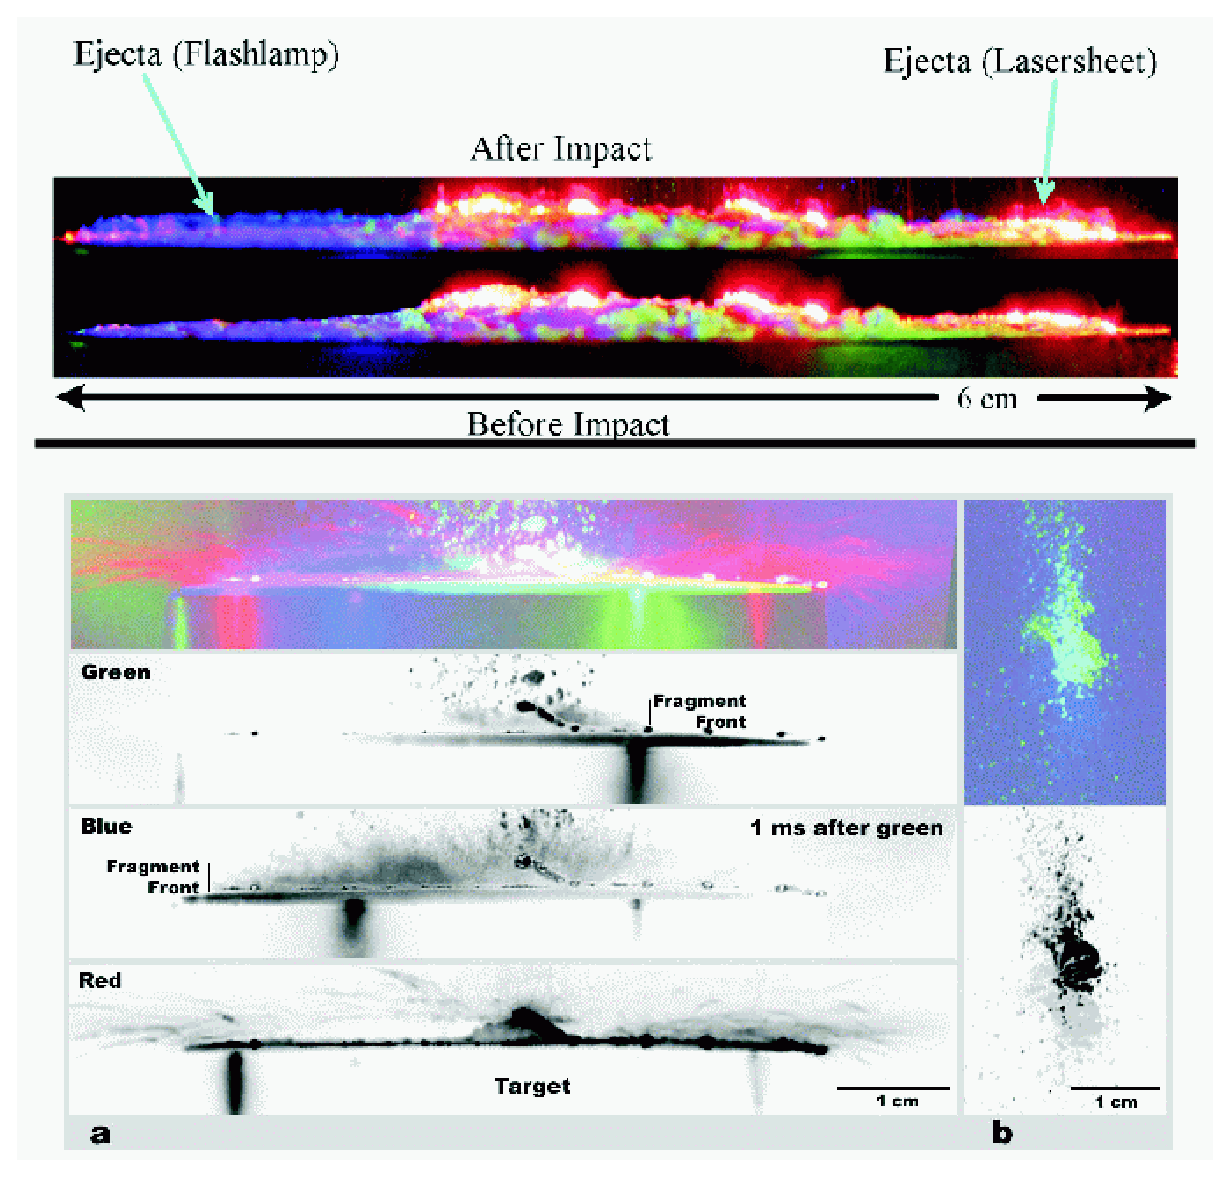
\includegraphics[width=15cm]{b2fig2.eps}}
\caption{\label{soorso}Outcome of a collision at $\rm >20m/s$. 
In the first (upper) case the collision is very destructive (Wurm et
al.~2005a). In the second (lower) case net growth occurred (Wurm et
al.~2005b).  The only difference is the initial structure of the target.}
\end{figure}


So far nearly ideal conditions have been assumed for
collisions. Experimental studies and models were mostly aiming at the
question whether a collision can lead to growth at all. Only for the
initial stage of particle growth it has been shown that the particles grow
as cluster-cluster aggregates in a self-consistent way (Blum 2004). For
larger dust aggregates, as seen in figure \ref{soorso} the outcome of a
collision, i.e.\ growth or fragmentation, strongly depends on the history of
collisions for a given target later on. While constructive and destructive
collisions have been shown to exist, it remains unclear if one of these
types of collisions is typically determining the outcome of collisions of
larger bodies with smaller ones.




%
% Here follows the own refereed publications by the PIs in relation to
% the project proposed here.
%
\ownpubltitle{Own publications related to the Forschergruppe:}
%
% BELOW IS ONLY AN EXAMPLE OF TWO ENTRIES. SEE THE ADDITIONAL FILES
% SENT TO YOU WITH ALL THE REFERENCES FROM THE VORANTRAG
%
\begin{ownpubl}
\item Blum, J. and Schr\"apler, R. (2004) Structure and Mechanical Properties of
High-Porosity Macroscopic Agglomerates Formed by Random Ballistic Deposition,
\prl, \textbf{93}, 115503

\item Blum, J. (2004) Grain Growth and Coagulation, in: \textit{Astrophysics of Dust},
ASP Conference Series, Vol. 309 (Eds. A. Witt, G. Clayton and B. Draine),
369-391

\item Blum, J. and Wurm, G. (2000) Experiments on Sticking,
Restructuring and Fragmentation of Preplanetary Dust Aggregates.
\ica, \textbf{143}, 138-146

\item Blum, J., Wurm, G., Kempf, S., Poppe, T., Klahr, H., et al.
(2000) Growth and Form of Planetary Seedlings: Results from a
Microgravity Aggregation Experiment. \prl, \textbf{85}, 2426-2429

\item Dominik, C., Blum, J., Cuzzi, J.N., Wurm, G. (2006) Growth of Dust
as the Initial Step Toward Planet Formation. in: \textit{Protostars 
and Planets V}, (Eds. B. Reipurth, D. Jewitt, K. Keil).\\ 
  {\tt http://ifa.hawaii.edu/UHNAI/ppv.htm}

\item Heim, L.-O., Butt, H.-J., Schr\"apler, R. and Blum, J.
(2005) Analyzing the Compaction of High-Porosity Microscopic
Agglomerates, Australian Journal of Chemistry, \textbf{58(9)} 671

\item Paraskov, G.B., Wurm, G., and Krauss, O. (2006) Eolian Erosion of
Dusty Bodies in Protoplanetary Disks. \apj, (accepted)

\item Poppe, T., Blum, J. and Henning, Th. (2000) Analogous
Experiments on the Stickiness of Micron-Sized Preplanetary Dust.
\apj, \textbf{533}, 454-471

\item Wurm, G., Paraskov, G. and Krauss, O. (2005) Ejection of
Dust by Elastic Waves in Collisions between Millimeter- and
Centimeter-sized Dust Aggregates at 16.5 to 37.5 m/s Impact
Velocities. \phre, \textbf{71}, 21304

\item Wurm, G., Paraskov, G. and Krauss, O. (2005) Growth of
Planetesimals by Impacts at ~25m/s. \ica, \textbf{178}, 253-263

\item Wurm, G. and Blum, J. (1998) Experiments on Preplanetary
Dust Aggregation. \ica, \textbf{132}, 125

\item Wurm, G., Blum, J. and Colwell, J.~E. (2001) Aerodynamical
sticking of dust aggregates. \phre, \textbf{64}, 046301

\item Wurm, G., Paraskov, G. and Krauss, O. (2004) On the
Importance of Gas Flow through Porous Bodies for the Formation of
Planetesimals. \apj, \textbf{606}, 983

\item Wurm, G., Paraskov, G. and Krauss, O. (2005) Ejection of
dust by elastic waves in collisions between millimeter- and
centimeter-sized dust aggregates at 16.5 to 37.5 m/s impact
velocities. \phre, \textbf{71}, 21304
\end{ownpubl}
%
\section{Goals (Ziele)}
\noindent The project is supposed to close in on a typical structure of a
larger ($> 10$ cm) body in a protoplanetary disk at a certain
time. The main issues are:

\begin{itemize}
\item What is the porosity and detailed morphology of an evolving dusty body?

\item Is the mass distributed homogeneously inside a large body or
are there macroscopic voids or very compact compartments within
such a body?

\item Is the permeability of the body large enough to allow a
sufficient gas flow through it to accrete small fragments from a
collision?

\item What is the size distribution of fragments which form 
in a typical collision?
\end{itemize}

\noindent The "typical" structure might change as the whole particle
distribution evolves with time. Once the typical structure is
given, more complex questions can be asked on how even larger
bodies evolve, what the effect of particle drift of a body into a
different particle distribution at a different part of the disk
might be, and feedback can be given on how the particle
distribution itself evolves due to the average collision.


\section{Work schedule (Arbeitsprogramm)}
\subsection{Methods}
We will carry out laboratory experiments using the experimental setups in
M\"unster and Braunschweig. These setups allow carrying out individual
collisions of dust aggregates of different size, porosity, velocity, impact
angle. A principle sketch of an individual experiment can be seen in
Fig.\ \ref{aufbau} (left). The right image shows the new high velocity setup
using a cross bow launcher.  A plausible sequence of impacts of dusty
projectiles onto the same dusty target will be carried out to see how the
target evolves.

\begin{figure}
%\centerline{\includegraphics[width=12cm]{aufbau.eps}}
\centerline{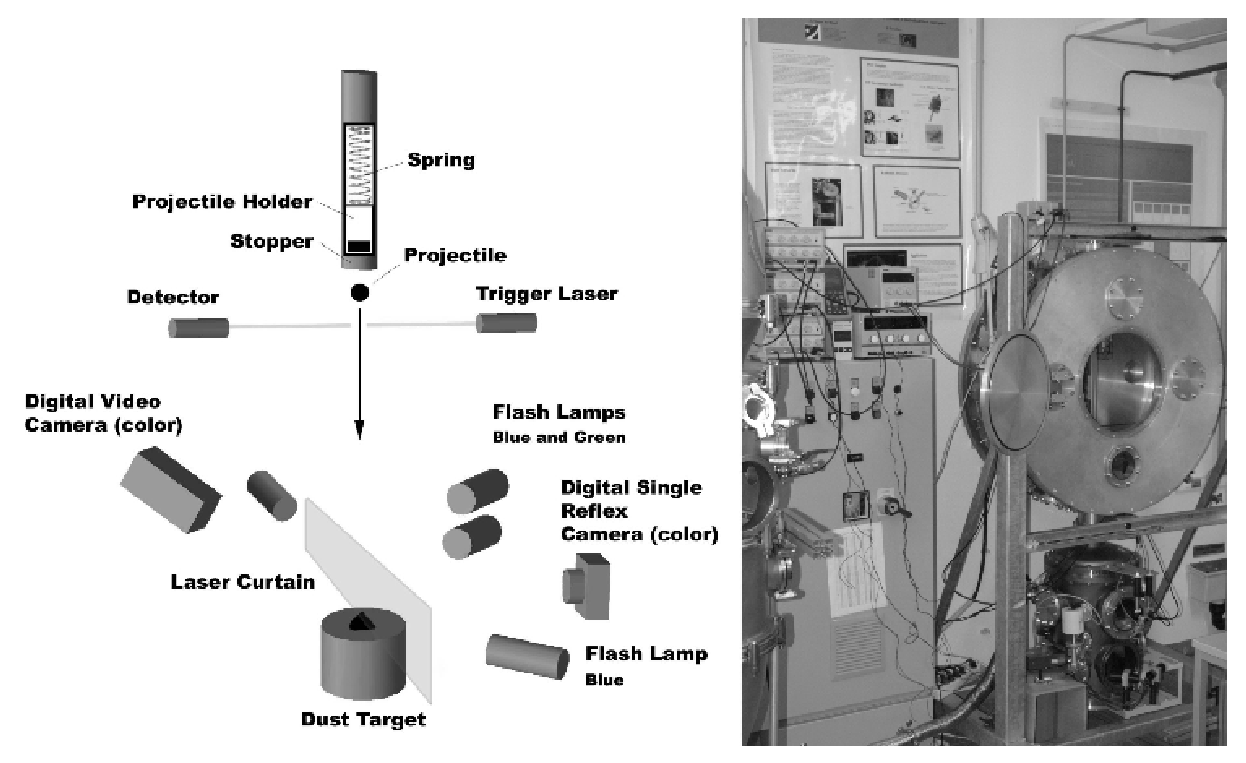
\includegraphics[width=15cm]{b2fig3.eps}}
\caption{\label{aufbau}(left) Principle of impact experiments as they have
been carried out in M\"unster.  (right) A new setup available at the
Institute of Planetology in M\"unster.  The upper right circular vacuum
chamber holds the cross bow launcher (100 m/s). The part below is the impact
chamber.}
\end{figure}


Initially different simple scenarios will be tested, e.g.\ a flat dusty
surface might be bombarded with large dust aggregates from different
arbitrary angles. We know that one dust projectile at high velocity leaves a
dust pile sticking to the target. We will study how the forming ragged
surface will react to more impacts from different angles. As addition of
individual dust particles or small aggregates at low collision velocity is
another mode of growth, we will alternatingly add layers of loose particles
and continue with large-aggregate impacts. Eventually, in an ideal case we
will carry out collisions of different kind in the sequence we expect them
under protoplanetary disk conditions. The input of the perfect sequence is
coming from the other projects within the research group, especially
\projdul{}.


Gravity is not negligible in all laboratory experiments, since the most
porous dust aggregates collapse under their own weight.  Compaction during
an impact might lead to the formation of an aggregate which is stable under
gravity.  Therefore, for collision sequences where intermediate states are
influenced by gravity, complex initial targets will be prepared artificially
to answer if e.g.\ hollow compartments below the surface are sustained after
an impact or collapse. The spatial extent of effects of a collision will be
studied. Data on individual collisions, i.e.\ size distribution of fragments
depending on the size, impact velocity, and porosity of the target body will
be distributed to the other members of the group in projects \projdul{},
\projkley{}, \projblum{}.  The fragments take part in the next
collisions. Therefore, the fragment distribution is one part of the
coagulation kernel (see \projdul{}) and determines how the size distribution
evolves over time. As all different kind of collisions happen at the same
time, it is non-trivial what collision sequence will be plausible. This
shall be closed in close collaboration with \projdul{}.

In addition, multiple impacts might be simulated in computer simulations in
project \projkley{}. This is especially important for the impact sequences
which are hardly accessible in laboratory experiments due to the strong
influence of gravity e.g for very large, very porous aggregates and high
collision velocities. Further experimental insight might be gained on
parabolic flights where ejecta are free to leave but where deceleration is
soft enough for the target to keep intact. This will allow a few ten
consecutive impacts onto one target in a single flight. Funding for such
flights will be requested elsewhere (DLR, ESA) during the course of this
project, which according to experience of past years will hopefully expand
the ground based data.

Where possible, targets will be analyzed with respect to their properties
like elasticity, sound speed, mass, morphology, porosity etc.  Some targets
will be prepared to characterize their inner morphology with respect to dust
distribution (e.g.\ pore size, local density). Analysis methods will range
from simple weighing, measuring surface morphology, analyzing morphological
changes with depth from 2-dimensional cuts to potential application of 3-D
imaging methods like X-ray or NMR Tomography in later years.

The change of permeability on a gas flow will also directly be measured in
the wind channel which is available in M\"unster.  To achieve this the
channel cross section is closed by a dust target with permeable bottom. At a
known flow rate of the wind channel and measured pressure before and after
the target the permeability can readily be obtained.  The morphology of an
evolving target will be modeled based on the results from the experiments
and calculations. This model target will be used to evaluate the flow of gas
through such a dusty body and the effect of re-accretion of dust particles.

\subsection{Schedule}
\subsubsection{First year}

In the first year first sequences of experiments with best assumptions on
dust targets and impacts will be carried out. A laser scanner will be
developed to measure the surface profile of an evolving target. To approach
a larger number of collisions simple sequences will be carried out
first. Based on their outcomes, more complex targets will be prepared to
serve as next initial target. The collisions will use the cross-bow launcher
in M\"unster and reservoirs of individual dust particles as currently
provided by a cogwheel disperser in Braunschweig. That way, collisions of
large aggregates but also phases of individual particle accumulation can be
simulated on one target. Experiments can be started as soon as the proposed
position is filled since the hardware exists and only minor adjustments are
needed.

The resulting data, e.g.\ fragment size distribution, target porosity and
cratering details will be distributed to the other groups \projblum{},
\projdul{}, and \projkley{}.  This data can be used to calculate a more
realistic size distribution (\projdul{}), to improve the simulation of
collisions and calibrate simulations which are not possible in the
laboratory (\projkley{}), and to give further input for charging experiments
(\projblum{}).  The discussion and feedback from the other groups will be a
continuous process also in the following years. Experimental results will be
fed to computer simulations while the numerical simulations in turn
determine the typical collision sequences which will be carried out in
experiments.


\subsubsection{Second year}

In accordance with the philosophy mentioned before, more realistic
collision sequences will be explored as the project proceeds. This
might not be divided in years but will evolve.

However, after the initial collision experiments permeability measurements of
typical dust targets will be carried out in the wind channel in
M\"unster. The effect of porous gas flow will be quantified and re-accretion
of particles by gas flow will be reevaluated as one source for mass gain and
surface sculpturing.

Microgravity experiments will be conducted to estimate the effect of gravity
on the impacts and the effect of elastic waves after impact into free
floating targets by observing fragments significantly away from an impact
side. This should finally lead to a formulation of an ever more realistic
description of the typical large dusty body in an evolving disk.

\subsubsection{Third year}

A database of collisions will be set up to provide the basic parameters of a
collision.  Ongoing collision experiments and gas flow experiments together
with a feedback of numerical coagulation studies (\projdul{}) should have
resulted in a more condensed view on the evolution of a larger body. The gas
flow measurements will be complemented by computer models of gas flow
through porous bodies, using commercial software (Femlab). This will be
based on recent simulations which have been carried out in M\"unster by
Paraskov et al.~(2006).  Eventually the description of a typical large body
should be defined in terms of morphology, i.e.\ density, porosity, pore
sizes, surface structure, tensile strength, elasticity, thermal properties,
etc..


\subsection{Literature}
%
% Here follows a general literature list related to the topic of the
% proposal, just like a literature list for a scientific paper.
%
% AGAIN ONLY EXAMPLES ARE LISTED NOW
%
\begin{literature}


\item Cancelliere, A., Chang, C., Foti, E., Rothman, D.H., and Succi, S. (1990) The
Permeability of a Random Medium: Comparison of Simulation with Theory,
\textit{Phys. Fluids A}, \textbf{12}, 2085

\item
Colwell, J. E. (2003)
Low velocity impacts into dust: results from the COLLIDE-2 microgravity experiment \ica, 
\textbf{164}, 188

\item
Colwell, J. E. and Taylor, M. (1999)
Low-velocity microgravity impact experiments into simulated regolith \ica, 
\textbf{138}, 241

\item Dominik, C. and Tielens,  A.~G.~G.~M. (1997) The Physics of
Dust Coagulation and the Structure of Dust Aggregates in Space
\ica, \textbf{480}, 647

\item
Hartmann, W. K. (1978)
Planet formation - Mechanisms of early growth \ica, \textbf{33}, 50

\item Koponen, A., Kataja, M., and Timonen, J. (1997) Permeability and Effective
Porosity of Porous Media \textit{PR E}, \textbf{56}, 3319

\item
Reynolds, O. (1885) On the dilatancy of media composed of rigid particles in contact 
\textit{Phil. Mag. Ser. 5}, \textbf{50}, 469 

\item Sekiya, M. and Takeda, H. (2003) Were planetesimals formed
by dust accretion in the solar nebula? \textit{Earth, Planets and
Space\/}, \textbf{55}, 263

\item Sekiya, M. and Takeda, H. (2003) Does the gas flow through
a porous dust aggregate help its growth in a protoplanetary disk?
\ica \textbf{176}, 230

\item Weidenschilling, S.~J. (1997) The Origin of Comets in the
Solar Nebula: A Unified Model \ica \textbf{127}, 290

\item Weidenschilling, S.~J. and Cuzzi, J.~N. (1993) Formation of
Planetesimals in the Solar Nebula. In: \textit{Protostars and
Planets III} (Eds. E.~H. Levy, J.~I. Lunine) University of Arizona
Press, Tucson, 1031

\item Further general literature on planetesimal (planet) formation relevant to the
project is given within the common list for the reserach group. 
 
\end{literature}



\section{External/International collaborations}
\begin{collablist}
\item[M\"unster] The IfP will be the host institute for the impact experiments.
Most experimental work and modelling of gas flows will be carried out
here. The project has access to the local facilities (see below) and technical 
support (technicians, workshop) by the department.
\item[Braunschweig] Some hardware is shared between M\"unster and
Braunschweig, e.g.\ high-speed cameras and illuminations or the
cogwheel dust disperser. A prototype of the anticipated laser
scanner was developed in Braunschweig and shall be used as the
baseline for the experiment-specific surface scanner. In addition
to that, porous dust aggregates as initial condition will be
generated in Braunschweig. 
\item[T\"ubingen] Data about the outcome
of the impacts will be compared to computer simulations done by
this group. Eventually multiple impacts not feasible in the
laboratory might be simulated complementing the experimental
results. 
\item[Heidelberg] More information about the motion and
coagulation of particles in (turbulent) disks will be provided by
these groups which will enable a better setup of collision
sequences. 
\item[Dr. J. Colwell, Boulder, USA] Dr. Colwell has
experience in collisions as well as was part in past activities of
gas aided re-accretion of dust particles. This experience will go
into determining the most realistic collision sequences and the
analysis.
\end{collablist}



\section{Link to other projects of the Forschergruppe}
\begin{linkproj}
\item[\projblum{}] As both re-accretion scenarios for dust
particles, electrostatic in project \projblum{} and aerodynamic in
project \projwurm{}, will influence the morphology of the growing
dust aggregates, a strong link between these two projects is
essential and will be established.

\item[\projkley{}] Results of the impacts will be compared with project
\projkley{} which performs numerical simulations of individual collisions of
porous bodies. On one side the experiments provide data as input for the
simulations. This might be used to reduce the free number of parameters in the
numerical models. On the other side the outcome of several collisions simulated
might provide initial conditions for further experiments and might expand
the region of collision sequences to parameters not accessible by laboratory
experiments.

\item[\projklahr{}] Project \projklahr{} can provide input on the typical
impact velocities expected. Since this is a free parameter in the experiments this
will also help restricting possible collision sequences better.
\item[\projdul{}] Project \projdul{} can predict which sequence of collisions
between which kind of bodies take place. The project will use the experimental results
to build a collision kernel and again to reduce the number of free parameters.
Eventually, after several feedback
loops, a more consistent picture of the typical dusty body should result.
\end{linkproj}



\section{Team members (Zusammensetzung der Arbeitsgruppe)}
%
% NOTE: Only list non-DFG-funded team members.
% NOTE: Also list technical assistants, students etc involved in the project
%
\begin{teamlist}
\item[Wurm, G., Dr. (Emmy Noether research group)]\mbox{}\\
Team leader; The project will be based on his experience in collisional physics for
planetesimal formation and the setups in his laboratory located in M\"unster.
\item[Blum, J., Prof.~Dr. (C3)]\mbox{}\\
Co-leader; Common experiment campaigns will be organized between Braunschweig and M\"unster.
\item[Krau{\ss}, O., Dr.]\mbox{}\\
Dr. Krau{\ss} is involved in the collision experiments in the laboratory in M\"unster.
He will actively take part in the experiments.
\item[Kley, W., ~Prof.~Dr. (C4)]\mbox{}\\
An intense collaboration is necessary to simulate collisions as well as to provide parameters
for experiments.
\item[Klahr, H., Dr.]\mbox{}\\
Work on possible particle/velocity distributions will provide better parameters for the
collision experiments.
\end{teamlist}
\vspace{1em}



\section{Funding requested}
The following table gives the full overview of requested
funding:\vspace{1\baselineskip}\\
%
% The table that follows is the overview over the full requested
% funding, including the positions, travel, consumables and ``other
% costs'' (which might include transportation costs of radioactive
% material or the rent of a drop tower or such).
%
\centerline{\begin{tabular}{||l|r|r|r||} \hline \hline & Year 1 & Year 2 &
Year 3 \\ \hline %
Personnel          & \hfil 24.000 &  24.000 &  24.000 \\
Consumables                        & \hfil 1.240 & \hfil 1.240 & \hfil 1.240 \\
Travel                             & \hfil 3.810 & \hfil 3.810 & \hfil 3.810 \\
Other costs                        & \hfil 1.000  & \hfil     & \hfil     \\
\hline
{\bf Total:}                       & \hfil 30.050 & \hfil 29.050 & \hfil 29.050 \\
\hline
\hline
\end{tabular}
}
\vspace{1em}\\
Below these costs are explained in more detail:

\subsection{Personnel (Personalbedarf)}
\begin{teamlist}
\item[PhD-Student (E13/2)]\mbox{}\\
While the setups for the experiments exist a dedicated project for multiple impacts requires
a person working on this full time. The experiments can best be carried out and analyzed
by a PhD student.
\end{teamlist}

\subsection{Consumables (Verbrauchsmaterial)}

For three years the following consumables are needed
\begin{itemize}
\item Oil for vacuum pumps 40 EUR/yr.
\item 300 arrows for launcher (a 5 EUR) which is 1 per experiment or
1500 EUR in total. 
(Arrows are destroyed each time due to the hard stop that ejects the dust.)
\item Material for mechanical workshop for small experimental adjustments at an estimated
500 EUR per year.
\item A few kg of dust for the experiments are estimated to 200 EUR/yr.
Since the project aims at a
self-consistent morphology we will initially use irregular dust, not special spherical particles.
\end{itemize}

\noindent
Estimated costs:\vspace{1\baselineskip}\\
 
\centerline{\begin{tabular}{||l|r|r|r||} \hline \hline & Year 1 & Year 2 &
Year 3 \\ \hline %
Oil               & \hfil     40 &     40 &  40 \\
Arrows (launcher)                  & \hfil 500 & \hfil  500 & \hfil   500 \\
Workshop                           & \hfil   500 & \hfil   500 & \hfil   500 \\
Dust                            & \hfil  200  & \hfil 200 & \hfil 200 \\
\hline
{\bf Total:}                       & \hfil  1.240 & \hfil  1.240 & \hfil 1.240 \\
\hline
\hline
\end{tabular}
}


\subsection{Travel expenses in addition to Project Z (Reisekosten)}
%
% Here only travel expenses not related to usual regular Forschergruppe
% meetings and the overall per capita budget for conferences.
%

The project requires two 2-day visits to or from T\"ubingen, Braunschweig,
and Heidelberg per year to discuss further proceedings or preparatory work.
For two persons travelling a 150 EUR (train), 70 EUR (Hotel one night) and
~30 EUR per diem (2 full or half days), this is 250 EUR per person or a total of 1500 EUR per year.


Common experiments require longer stays in Braunschweig or visits from Braunschweig.
We estimate these to be 3 weeks per year. Each week is about 300 EUR for travel
(incl. experiment hardware transport), 5 nights a 70 EUR (one person), 5 days per diem
a 24 EUR or a total of 770 EUR per week, a total of 2310 EUR per year.

Estimated costs
are:\vspace{1\baselineskip}\\
\centerline{\begin{tabular}{|p{18em}|p{7em}|p{7em}|}
\hline
& \hfill per year EUR& \hfill total EUR\\
\hline
Regular meetings & \hfill 1.500 & \hfill 4.500\\
\hline
Experiment campaigns & \hfill 2.310 & \hfill 6.930\\
\hline
\end{tabular}}


\subsection{Other costs (Sonstige Kosten)}

As small equipment a laser diode (line) is needed to set-up a laser scanner
for determination of the surface morphology. Estimated costs (catalogue) 1.000 EUR
in the first year.
%%%  For publication in ApJ 500 EUR are estimated in year 2 and 3.

%% Estimated costs:\vspace{1\baselineskip}\\
\centerline{\begin{tabular}{|p{15em}|p{10em}|p{7em}|}
\hline
  & \hfil  & \hfil total EUR \\
\hline
Laser&& \hfill 1.000\\
%% \hline
%% Publications&& \hfill 1.000\\
\hline
\end{tabular}}




\section{Preconditions for carrying out the project at home institution}
%
% This is one of the main subsections of a DFG Normalverfaren proposal.
% Several of the subsubsections in this subsection we have placed in their
% own subsections above (like team members, collaborations). What remains
% are the following three subsections. For those not familiar with these,
% we refer to the DFG Merkblatt on Normalverfahren-proposals.
%
\subsection{Scientific equipment available (Apparative Ausstattung)}
%
% Please list those larger instrument available to you for the project (if
% applicable also larger computer equipment in case you need substantial
% amounts of computer time).
%
\begin{itemize}
\item In M\"unster the experimental setups for individual collisions between mm and dm size
dust aggregates exist and can be used. This includes flash lamps, cameras, vacuum equipment, launcher,
scales, etc.

\item Computers for data analysis exist.

\item A wind channel for gas flow experiments dedicated to this kind of work can be used in
M\"unster.

\item Software (Femlab) for numerical calculations of gas flow, including gas
flow through porous dusty bodies also exists.

\item The project has access to the analytical instruments being part of the Institute
of Planetology and Earth science department like optical microscopes and scanning
electron microscope, which can e.g.\ be used to characterize dust samples with respect
to size distribution.

\item High-speed cameras and high-speed flash-lamp illumination
will be made available to the project by the Braunschweig
laboratory.

\item The Braunschweig cogwheel dust disperser will be used for
sample preparation as well as for multiple-impact experiments in
M\"unster.

\end{itemize}


\subsection{Institution's general contribution (Laufende Mittel f\"ur Sachausgaben)}
%
% Please state the annual fund for consumables which comes from the
% institution's budget or any other third party  (please list separately) to
% pay for the research for which your project is part of.  Use estimates where
% applicable.
%

The project will be supported with about 500 EUR per year.


